%!TEX root = ../main.tex
\setcounter{chapter}{1}
\chapter{Control and observation}
In this session we tackle the design of an LQR controller and apply them to our path tracking problem.
The general idea is using the \emph{discrete-time linear model} of the system to design an LQR controller that will be used to control the \emph{nonlinear system}. 
Then, the LQR will be complemented with an observer that will use the model of the system to reconstruct one non-measured state. 

% \par
%
% One Simulink diagram will be completed in this session, and it will include both the control and the observation stages. 
\section{Provided files}
\begin{itemize}
	\setlength\itemsep{0em}
	\item \texttt{LQR\_observer.slx}.
		A simulink files with some of the blocks needed to simulate the system + controller + observer combo.
	\item \texttt{ex2.m}.
		The class whose methods have to be completed.
		A description of every function to be completed is included within the file.
	\item \texttt{exercise2\_LQRandObserver.m}.
		The Matlab script which sets and runs the required simulations.
		Modify its content only if you want to run other experiments in addition to the ones proposed.

		\note{Note that although you will be modifying methods in the \texttt{ex2.m} class, it is the \texttt{exercise2\_LQRandObserver.m} script the one that you have to execute to run the proposed experiments and simulation. }		

	\item \texttt{utilities.m}.
		The class which gathers auxiliary functions that will be used in the scripts provided during the case study sessions.
		There is no need to review its content unless you want to make use of some of the functions included therein.
	\item \texttt{circle, path\_1, path\_2, path\_3} mat files containing different paths to track that can be used in the experiments.
\end{itemize}



%
\section{Exercises}
	\paragraph{Transfer your solutions from the first session:}
	\begin{enumerate}
		\item Place within the Matlab's working directory the class \texttt{ex1.m} with your solutions to the exercises proposed in the first case-study session. 
	\end{enumerate}
	\paragraph{LQR design:}
	\begin{enumerate}
		\setcounter{enumi}{1}
		%
		\item Complete the method \texttt{getLQRCostFunctArrays} for it to return the matrices %
		\begin{align}
			Q_1 & = \matriz{ccccc}{
				0.00001 & 0 & 0 & 0 & 0 \\
				0 & 50 & 0 & 0 & 0 \\
				0 & 0 & 0.5 & 0 & 0 \\
				0 & 0 & 0 & 0.5 & 0 \\
				0 & 0 & 0 & 0 & 0.5
			} & 
			Q_2 & = \matriz{cc}{
				1 & 0\\
				0 & 0.00002
			}
		\end{align}
		defining the cost function of the optimal control problem. 

		\item Complete the method \texttt{getLQRGain} where the LQR gain will be calculated by solving the Ricatti equation iteratively.

		\note{
			The number of iterations required to obtain $S_\infty$ will be obtained through trial and error.
			It must be sufficiently large so that $S$ converges. This condition can be observed, for instance, by keeping track of the singular values of $S$ (which would as well converge with $S$). 
		}
	\end{enumerate}

	\paragraph{State observer design and implementation}
	Once the LQR controller has been calculated, we will design an observer. 
	To do so, we first need to change our assumption concerning the system's output equation since, if we continue considering the system's output to be 
	\begin{align}
		\mathbf{y} = \mathbf{x}
	\end{align}
	all states would be available and thus an observer would not be necessary\footnote{This is not totally true as an observer might as well be useful in scenarios where the full state vector is available and the system's initial state is unknown and/or the signals are affected by noise.}. 

	For this reason, the first step consists in choosing an \emph{alternative} system's output %
	$\mathbf{y}'$, %
	given by the equation
	\begin{align}
		\mathbf{\tilde{y}}'(k) = C' \mathbf{\tilde{x}}(k) = C'\mathbf{\tilde{y}}(k)
	\end{align}
	so that the system's output become 
	\begin{align}
		\mathbf{\tilde{y}}'(k) = \trasp{\left[x_1(k), x_2(k), x_4(k), x_5(k) \right]}.
	\end{align}
	Then, our observer will have to generate the estimated state vector $\hat{\tilde{\mathbf{x}}}(k)$ given the output $\mathbf{\tilde{y}}'$.

	\begin{enumerate}
		\setcounter{enumi}{3}
		\item Complete the method \texttt{alternativeSystemsOutputEquation}, which returns the array %
		$C'$ %
		defining the system's alternative output equation we will use to justify the use of an observer. 
		
		\item Complete the method \texttt{checkObservability} where you will assess whether the system is observable or not. 
		
		\note{To calculate the observability matrix, you can use the matlab command \texttt{obsv}.}

		\note{Here you need to take into account the \emph{alterantive} output equation.}
		%
		\item Complete the method \texttt{getObserverGain} where the observer gain is calculated.
		Start by setting the poles of the observation loop as the %
		$99.9\%$ %
		of the poles of the closed control loop. 

		\note{Remember that the eigenvalues of the control closed loop are given by %
		$\texttt{eig}(\Phi - \Gamma * lqr_K) $ }

		\note{
            To calculate the observer gain, use the matlab command \texttt{place}. 
            Read the help information and notice that the function is meant to be used to calculate control gains.
            That is it returns gains to impose certain poles assuming that the closed loop dynamics is given by (A-B*K). 
            However, we want to use to to place the poles of the observer. 
            Check and compare the observer close loop, build a parallelism with the control case, and introduce the needed modifications in the matrices given to the \texttt{places} method. 		
		}

		\item Complete the method \texttt{getObserverInitialState} that returns the state that the observer will initially assign to the states it has to observe. 
		You can choose the first guess of the observer freely and it may differ from the system's real initial state. 
	\end{enumerate} 

\section{Simulink diagram and simulation}
	Once we have the LQR controller and the observer designed, you will complete one Simulink diagram allowing us to close the control loop in two different ways.
	A draft schematic that illustrates the task is provided in Fig.\ \ref{fig:simulinkDraft}.
	The idea is including a switch in the scheme allowing us to close the control loop with the initially assumed system's output %
	$\mathbf{y}$ %
	or the alternative output $\mathbf{y}'$.
	\begin{figure}[!h]
		\centering
		\resizebox{ 250 px }{!}{
			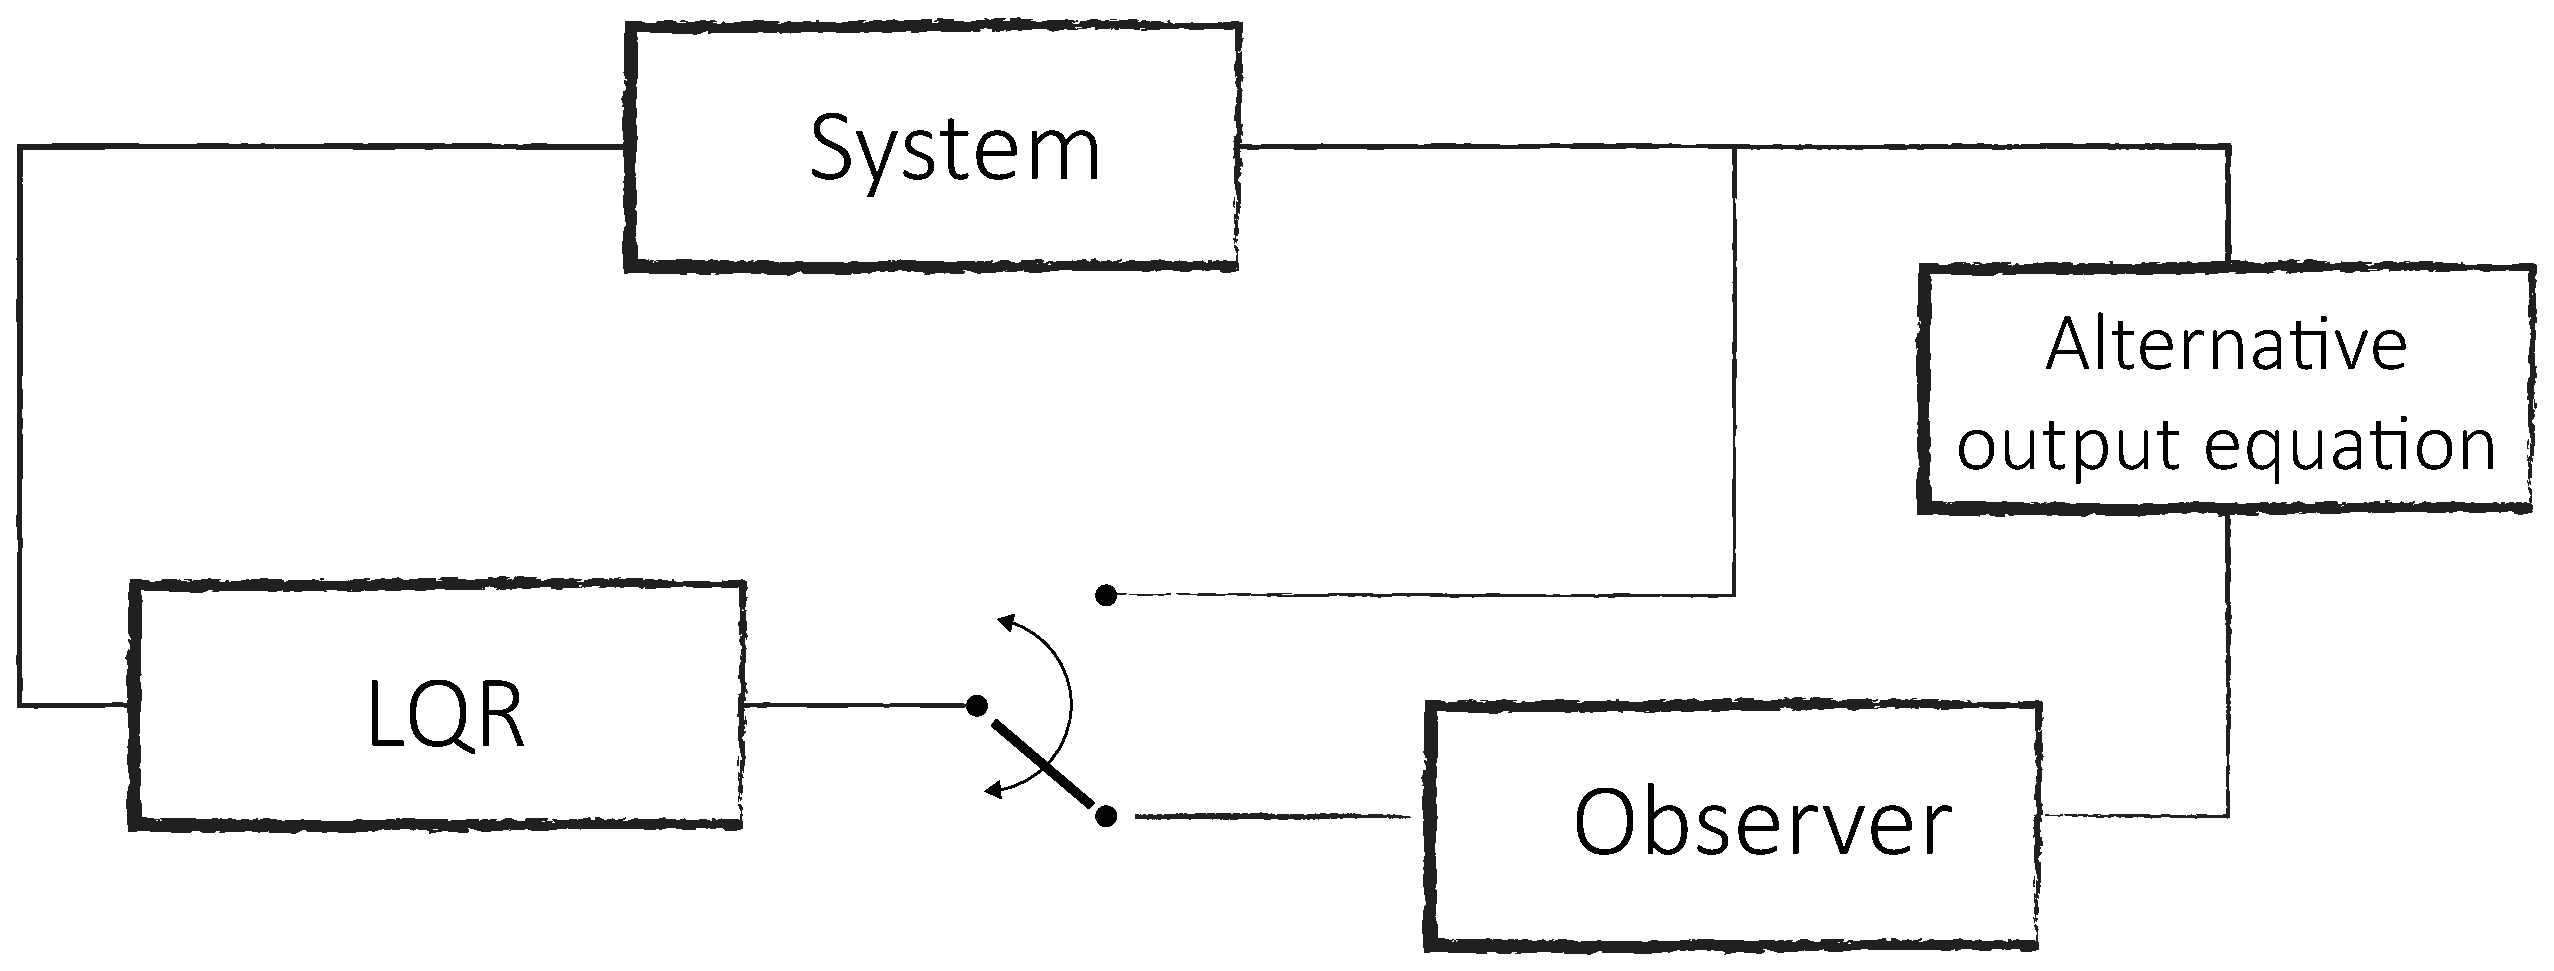
\includegraphics[width = 250px]{./_imags/draft_observer_scheme}
		}
		\caption{Draft of the targeted simulink diagram.}
		\label{fig:simulinkDraft}
	\end{figure}	

	\begin{enumerate}
		\setcounter{enumi}{7}
		\item Complete the Simulink diagram \texttt{LQR\_observer.slx} given the information provided above. 
		
		\note{Several \emph{subsystem} blocks are included in this Simulink file. 
		Explore all of them to identify the ones you need to complete.}

		\note{The observer is to be implemented using a state-space block. A example of how this should be done is provided in exercises 6.6.1-3. }

		\item Complete the method \texttt{getObserverImplementationArrays} where the arrays %
		$AObs$, %
		$BObs$, %
		$CObs$, and %
		$DObs$  %
		needed to implement the observer with a state-space block are calculated.
	\end{enumerate}

\section{Questions}
	\begin{enumerate}
		\item Report the value of the LQR gain for the proposed $Q_1$ and $Q_2$, as well as the evolution of the singular values of $S$ obtained while solving the Riccati equation.
		\item Report the explicit value of the observation close loop poles, and the observer gain resulting from it. 
		\item Provide a screen shot of your final Simulink scheme and the submodules you had to complete. 
		\item Report the simulation results for the proposed values. 
		\item The proposed value of $Q_1$ intends to assign very little importance to the error deriving from $x_1$. Could you explain why doing this might make sense? 
		\item Propose a different pair $Q_1$ and $Q_2$ such that heading deviation error is highly penalized compared to the other states and report simulation results where the impact of doing so can be clearly observed. 
		\item Is the proposed placement for the observation close loop poles appropriate? why? If not, propose a new set of poles to improve the observation performance.
	\end{enumerate}